\section{Limitation of Past Surveys}\label{sec:past_detection_context}
   
   What is apparent from the plethora of debris disk studies over the last three decades is the differences in the reported incidence rate of excesses. Though there is a consensus within the community in terms of typical rates for a given spectral type at rough ages, the differences, even within these bins, cannot be ignored in the larger context of this thesis. 
   
   There are a few reasons why these differences exist. The first is instrument sensitivity. Different instruments aboard these satellites are sensitive to a certain degree. A good review can be found in \citet{Wyatt2008}, where Dr. Wyatt describes the limiting fractional excess $R_{\lambda,\rm{lim}}$ above which a disk is detectable, typically calculated based on the limits of the faintest disk detected in the survey. Thus, equation 11 in \citet{Wyatt2008} defines the lowest fractional luminosity above which a disk is detectable such that
   
   \begin{equation}\label{eq:detection_limits}
   f_{\rm{det}} = 6\times10^9 X_\lambda \frac{R_{\lambda,{\rm lim}}L_\star}{r^2 T_\star^4} \frac{B_\lambda(T_\star)}{B_\lambda(T_d)}. 
   \end{equation}
   
    %===================================================================
    %  DISK DETECTION
    %===================================================================
    \begin{figure}
    \centering
    \begin{tabular}{cc}
    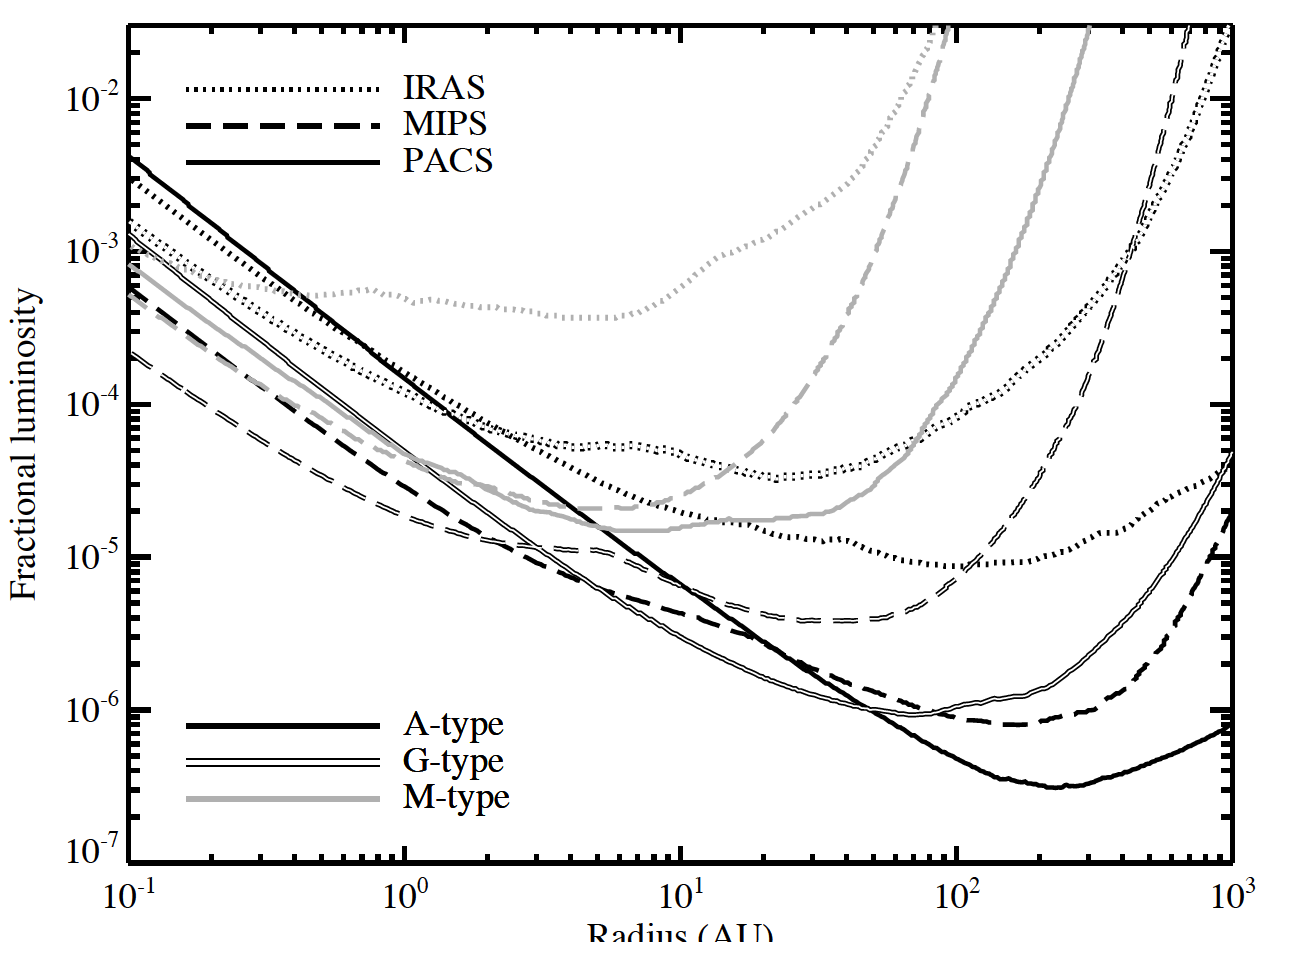
\includegraphics[scale=0.2]{Ch2/Detection_limits_Kennedy} &
    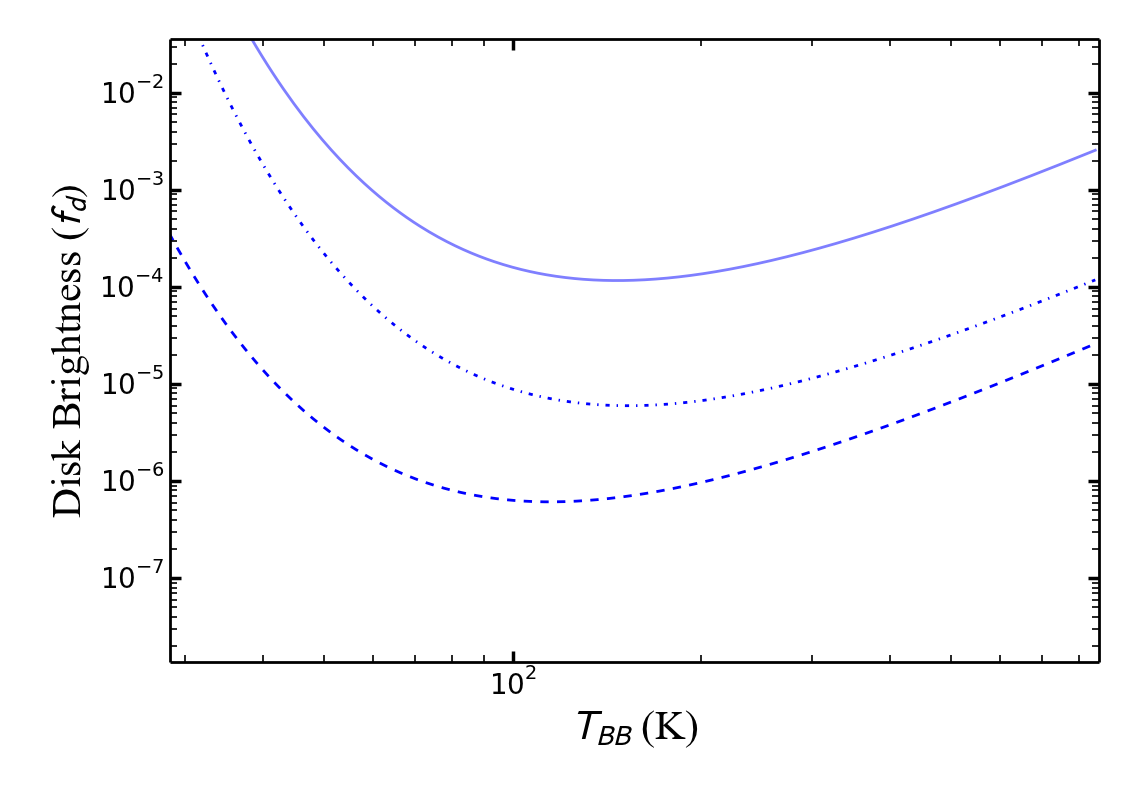
\includegraphics[scale=0.3]{Ch2/fd_vs_tbb_simple}
    \end{tabular}
    \caption[]{}
    \label{fig:detection_limits}
    \end{figure}
    %===================================================================
    
   
   The left panel of Figure~\ref{fig:detection_limits} shows the limiting fractional luminosity a few different surveys as a function of radius from the star. From IRAS to Herschel, improvements in both detector technology and an increase in mirror size have pushed the limits of detecting fainter and fainter dust populations. Hence, the increase of incidence rates from IRAS to Spitzer does not come as much of a surprise given that Spitzer is sensitive to fainter dust (cold or warm). Differences in incidence rates can also arise due to the threshold of an excess some studies may adopt compared to others. 
   
   As explained in \S~\ref{sec:excess_resolvedimaging}, the excess flux is measured from the measured IR flux subtracted from the photospheric flux in the IR, which is extrapolated from model fits to optical and near-IR flux measurements. Studies may determine the significance of an excess detection from this subtraction on a case by case basis, or from the statistical significance based on the distribution of a large survey. The former method can under or overestimate the excess if significant flux variations occur between the epoch of observations between the optical data and the IR data, while the latter technique may introduce large false-discovery rates \textbf{check this} as well as reduce the sensitivity of fainter disks for small samples in a survey. 
   
   Studies that used some of the more notable space based observatories like Herschel or Spitzer were limited to sample sizes of $\sim$500 stars, due to the pointed nature of the satellite. And although IRAS was an all-sky mission, it also produced a couple hundred excess sources. The study by \citet{Rhee2007} searched for excesses around tens of thousands of Hipparcos main-sequence stars, and produced roughly 50 new excesses, the majority of which were still cold disk detections. We have seen that cold dust is easier to detect due to the large contrast with the photosphere in the far-IR. The contrast becomes an issue in the mid-IR, where there are a relatively low number of warm dust detections.
   
   The reason behind the overall low number of warm dust detections is because of the small coverage of very sensitive pointed satellites like Spitzer and Herschel, and the relatively low resolution and sensitivity of the last all-sky mission, IRAS, where the resolution of the IRAS beam was 30'' at 12\micron. Thus, to addresss the limitations presented, I now shift focus of this thesis to finding warm dust with the latest all-sky infrared mission: the Wide-Field Infrared Survey Explorer Spacecraft.
   
   
\section{The Wide-Field Infrared Survey Explorer\\ Mission}\label{sec:wise_intro}

    The success of the IRAS mission was one of the motivations for launching another new and improved infrared all-sky mission. The goals of the Wide-Field Infrared Survey Explorer mission \citep[WISE;][]{Wright2010} were to observe the entire sky at two near-IR and two mid-IR wavelengths, thus improving and complementing the achievements of IRAS. In this section, I discuss the details of the WISE mission. Data from the WISE survey constitutes the bulk of my thesis and in the the following section, I will summarize this space based mission, its purpose and the specifications and how its data products can be used to identify circumstellar dust.
   

    \subsection{Mission Overview}\label{sec:wise_overview}


    WISE is an Earth orbiting observatory, 525~km above the Earth's surface. WISE was funded by NASA/JPL and launched on December 14th, 2009. It is a medium-class explorer mission weighing 750~kg. The satellite consists of a 40~cm diameter telescope and four imaging CCDs which are cooled by solid hydrogen cryostats. Two of the CCDs are designed to image the sky in the near-infrared wavelengths (3.5\micron and 4.6\micron) and two in the mid-infrared (12\micron and 22\micron). Figure~\ref{fig:WISE_satellite} shows an illustration of the physical satellite. 
  
    
    %===================================================================
    %  WISE SATELLITE
    %===================================================================
    \begin{figure}
    \centering
    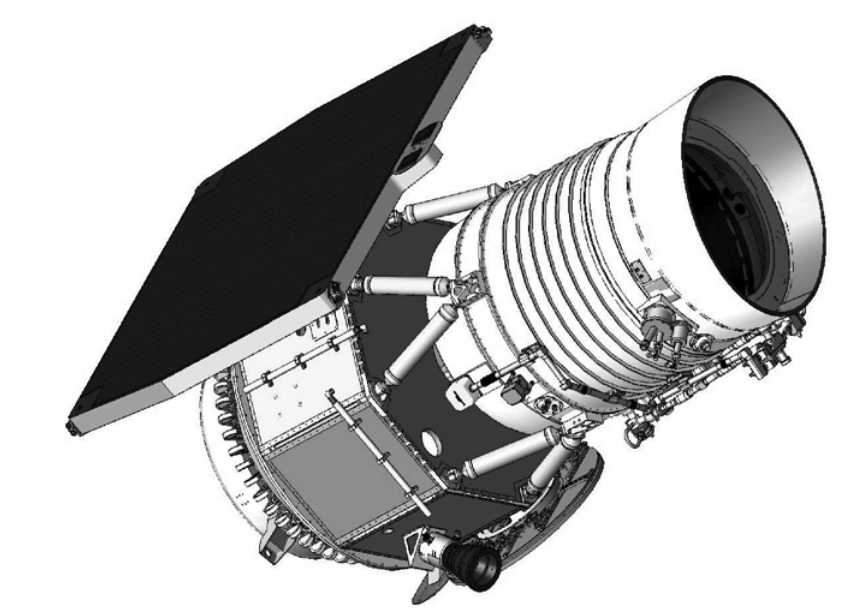
\includegraphics[width=\textwidth]{Ch2/wise_satellite}
    \caption[]{}
    \label{fig:WISE_Satellite}
    \end{figure}
    %===================================================================
    
 
    The mission was successful in scanning 99.99\% of the entire sky in the aforementioned IR bands. WISE's detector field-of-view is 47' on a side. During its continual orbit around the Earth, overlapping observation frames 11 second cadences were taken (8.8~s of integration). The overlap of frames, over multiple orbits, ensures greater depth of coverage. In a day, the satellite performs 15 orbits. Figure~\ref{fig:scan_plan} shows the overlapping frames as the satellite orbits the Earth. Further details of the entire mission can be found online\footnote{\url{http://wise2.ipac.caltech.edu/docs/release/allsky/expsup/}} or in \citet{Wright2010}. 

    %===================================================================
    %  WISE SCAN PLAN
    %===================================================================
    \begin{figure}
    \centering
    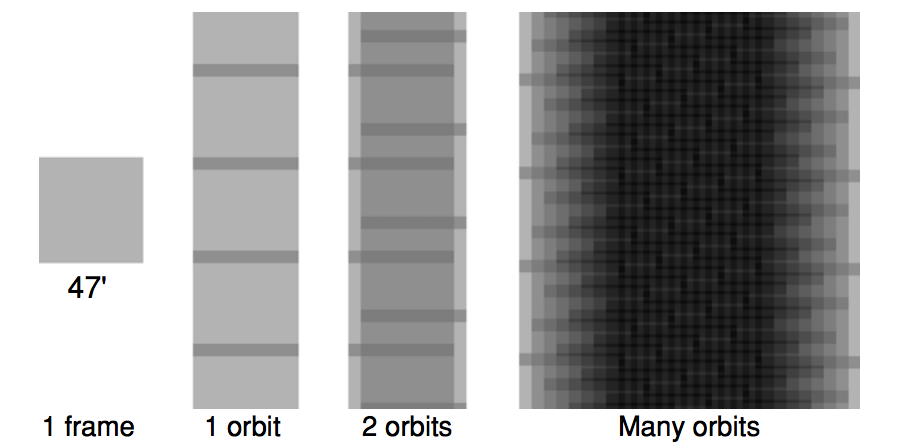
\includegraphics[width=\textwidth]{Ch2/wise_scan_plan}
    \caption[]{}
    \label{fig:wise_scan_plan}
    \end{figure}
    %===================================================================
    
    
   
   
    \subsection{WISE Bands}\label{sec:wise_bands}
   
   
   The two near-IR channels image the sky at band centered wavelengths of 3.4\micron\ and 4.6\micron\ using HgCdTe arrays, each with 18\micron\ 1024 $\times$ 1024 pixels. Both of these detectors are cooled to 32~K. The mid-IR channel detectors image the sky at band centered wavelengths of 12\micron\ and 22\micron\ and are made from Si:As BIB arrays of the same structure as the near-IR channels. These arrays are cooled to a temperature of 8.2~K. For the remainder of this thesis, I will refer to each of these bands as $W1$ (3.4\micron), $W2$ (4.6\micron), $W3$ (12\micron) and $W4$ (22\micron). Figure~\ref{fig:wise_bands} shows the relative spectral response of each of the detectors. 
   
    %===================================================================
    %  WISE BANDS
    %===================================================================
    \begin{figure}
    \centering
    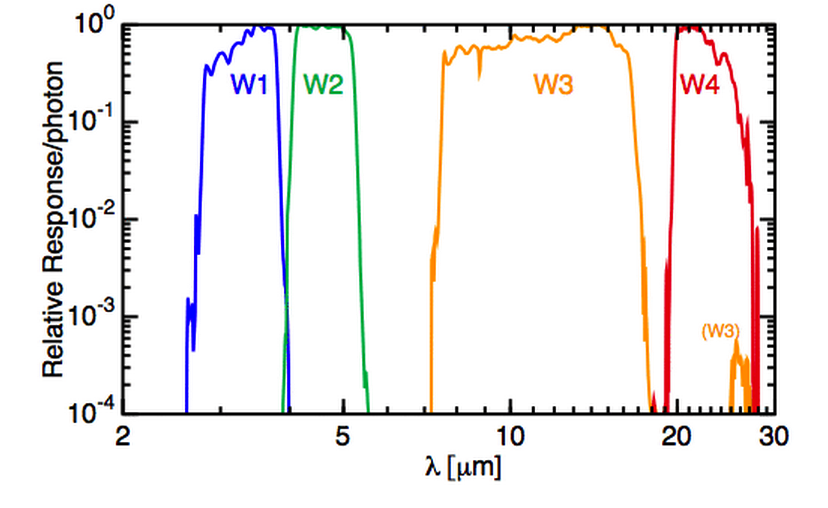
\includegraphics[scale=0.5]{Ch2/wise_response}
    \caption[]{}
    \label{fig:wise_bands}
    \end{figure}
    %===================================================================
    
    
   
    \subsection{WISE Data Products and the All-Sky Data Release}

    The WISE mission has produced a number of different data releases. The first release, called the \textit{WISE Preliminary Release} was made public on April 14, 2011\footnote{\url{http://wise2.ipac.caltech.edu/docs/release/prelim/preview.html}} and contained data that covered only 57\% of the sky. The next public release of WISE data was made on March 14, 2012. This data set was called the \textit{All-Sky Data Release}\footnote{\url{http://wise2.ipac.caltech.edu/docs/release/allsky/}} and covered the entire sky in all four bands. After the cryostats were depleted, WISE began its ``warm'' mission, and only collected data in the two near-IR $W1$ and $W2$ bands. This commenced the Near-Earth Object WISE (NEOWISE) mission. A subsequent all-sky data release by WISE came on November 13, 2013 called the \textit{All-WISE Data Release}\footnote{\url{http://wise2.ipac.caltech.edu/docs/release/allwise/}}. For the work I present in the rest of this dissertation, I only use measurements from the \textit{All-Sky Data Release}, except in comparison with other release. 
    
    Since the WISE data is in the public domain, it can easily be accessed online. The online databases consists of measurements for over half a billion objects in all four bands. These measurements consist of photometric data for each band, as well as meta-data pertaining to the quality of the data product. The database also consists of Atlas images of the processed data and can be viewed at \url{http://irsa.ipac.caltech.edu/applications/wise/}. 
    



    \subsection{Advantages Over Previous Debris Disk Surveys}

    As outlined in \S~\ref{sec:excess_resolvedimaging}, the search for an infrared excess requires precise and accurate measurement of the photospheric flux, an instrument which is sensitive to low levels of dust which is common for most debris disks ($f_\rm{d}\sim10^{-2}$), as well as the ability to discern whether the IR source detected is stellar or chance alignment. Otherwise
    
    
    The past debris disk surveys have quite well established the frequency of disks. For young stars, this incidence is relatively high ($\sim$50\% in some age groups), but as low as 20\%--30\% for intermediate mature stars for cold disk detections and as low as a few percent for warm disk incidences. Thus, identification of a large number of sources requi

    
    %===================================================================
    %  Mission Sensitivities
    %===================================================================
    \begin{figure}
    \centering
    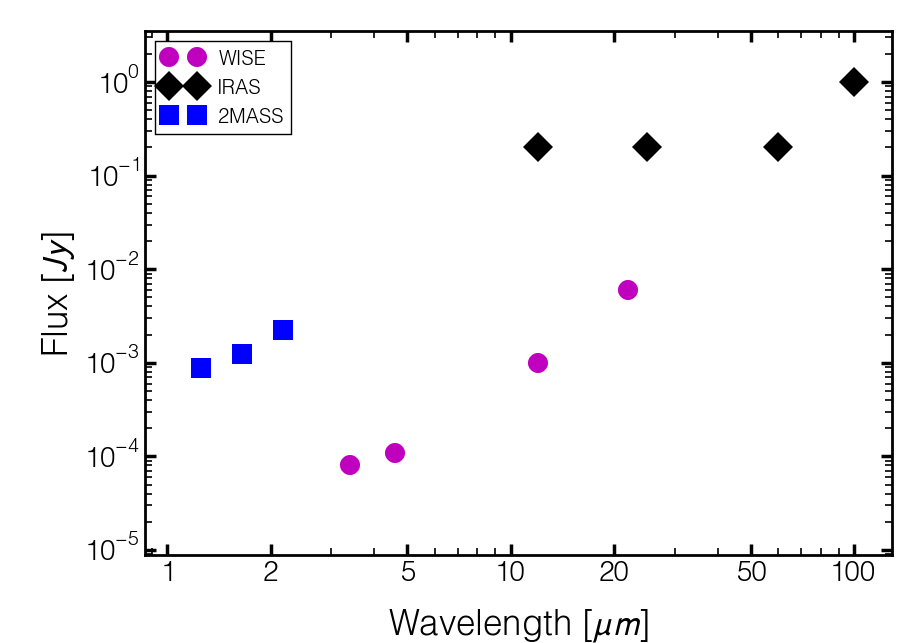
\includegraphics[scale=0.5]{Ch2/flux_density_comparison}
    \caption[]{}
    \label{fig:flux_comparison}
    \end{figure}
    %===================================================================
    
    
    
    
    
    
    %===================================================================
    %  IRAS vs. WISE
    %===================================================================
    %\begin{figure}
    %\centering
    %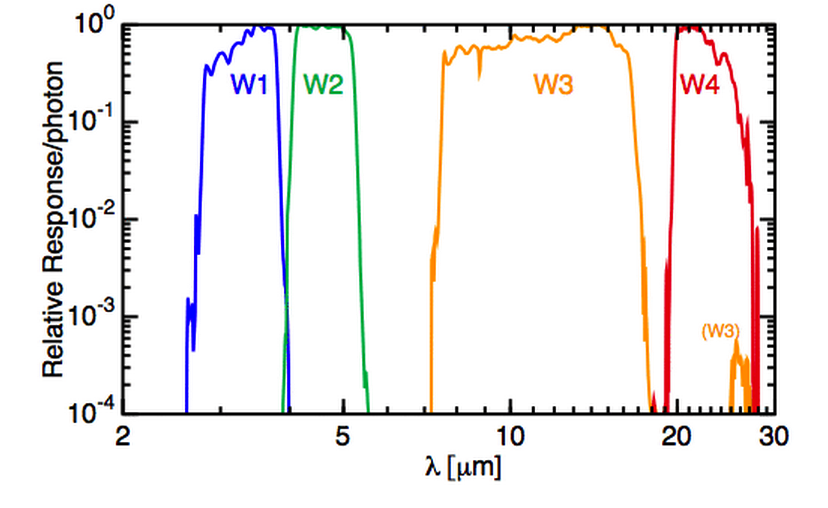
\includegraphics[scale=0.5]{Ch2/wise_response}
    %\caption[]{}
    %\label{fig:wise_bands}
    %\end{figure}
    %===================================================================
    
    